%=========================================================

% Here you can choose to compile with or without solutions.
% However, this definition is ignored if you use any
% command from the `Makefile`.
\providecommand{\withSol}{\iftrue}

%=========================================================

\documentclass[twoside,english,colorbacktitle,accentcolor=tud9c]{tudexercise}

\usepackage[T1]{fontenc}
\usepackage[latin9]{inputenc}
\usepackage{amstext}
\usepackage{amsmath}
\usepackage{graphicx}
\usepackage{setspace}
\usepackage{multicol}
\usepackage{mathtools}
\usepackage{dsfont}
\usepackage{units}
\usepackage{subfigure}
\usepackage{color}
\usepackage{booktabs}
\usepackage{fancyref}
\usepackage[ngerman,english]{babel}

%=========================================================

\def\homework{1}
\def\homeworkVer{1}
\def\homeworkSolVer{1}
\def\lecture{Statistical Machine Learning}
\def\semester{Summer Term 2021}
\def\prof{Prof. Stefan Roth, Dr. Simone Schaub-Meyer}
\def\deadline{Due date: 25. May 2018}

%=========================================================

\ifcsname withSol\endcsname\else
  \expandafter\let\csname withSol\expandafter\endcsname
                  \csname iffalse\endcsname
\fi

\withSol
	\usepackage[solutions]{iasHomework}
\else
	\usepackage{iasHomework}
\fi

%=========================================================

% USE YOUR NAMES!
\newcommand{\studentdata}{}
%\newcommand{\studentdata}{John Doe, 1234567 \qquad Jane Doe, 7654321}

\begin{document}
	
	\hwtitle{}
	\maketitle
	
	\begin{examheader}
		\normalsize
		\vspace{-1em}
		Stefanie Martin, Maximilian Nothnagel \hfill \studentdata{}
		\vspace{-1em}
	\end{examheader} 
	
	\textbf{Stefanie Martin, Maximilian Nothnagel \hfill \studentdata{}}
	\exercise{Machine Learning Introduction }
\begin{questions}
	
	%----------------------------------------------
	\begin{question}{Model Fitting }{6}		
	\begin{answer} 
	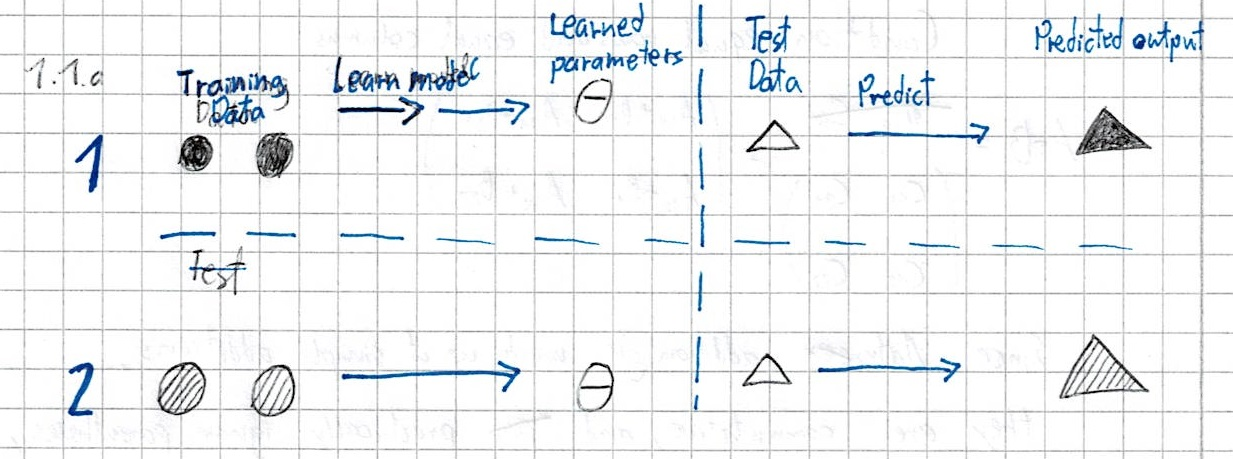
\includegraphics{1}\\
	Model 1 is being trained on filled circles, and as such assumes that the triangle is also to be filled, coming to an incorrect result.\\
	Model 2 is being trained on striped circles, and as such assumes that the triangle is also to be striped, coming to the correct conclusion.
		
	\end{answer}
		
	\end{question}
	
\end{questions}


	\exercise{Linear Algebra Refresher}
\begin{questions}
	
	%----------------------------------------------
	\begin{question}{Matrix Properties}{5}		
	\begin{answer} 
	\begin{enumerate}
		\item  Multiplication
	\begin{equation*} 
		A*B = 
		\begin{pmatrix}
			A_{1,1}*B_{1,1}+A_{2,1}*B_{1,2} & A_{1,1}*B_{2,1}+A_{2,1}*B_{2,2} \\
			A_{1,2}*B_{1,1}+A_{2,2}*B_{1,2} & A_{1,2}*B_{2,1}+A_{2,2}*B_{2,2}
		\end{pmatrix}
	\end{equation*}
	$A*B$ is defined only when Columns of B equal rows of A.\\
	\begin{equation*} 
		\begin{pmatrix}
			0 & 1 \\
			0 & 0
		\end{pmatrix}
		*
		\begin{pmatrix}
			0 & 0 \\
			1 & 0
		\end{pmatrix} 
		= 
		\begin{pmatrix}
			1 & 0 \\
			0 & 0
		\end{pmatrix}
	\end{equation*}
	BUT\\
	\begin{equation*} 
	\begin{pmatrix}
		0 & 0 \\
		1 & 0
	\end{pmatrix} 
	*
	\begin{pmatrix}
		0 & 1 \\
		0 & 0
	\end{pmatrix}
	= 
	\begin{pmatrix}
		0 & 0 \\
		0 & 1
	\end{pmatrix}
	\end{equation*}
	Matrixmultiplication is not Commutative.\\
	$A(B+C) = AB + AC$
	\begin{equation*} 
		\begin{pmatrix} %01
			0 & 1 \\	%00
			0 & 0
		\end{pmatrix} 
		*(
		\begin{pmatrix} %00
			0 & 0 \\	%10
			1 & 0
		\end{pmatrix}
		+ 
		\begin{pmatrix} %11
			1 & 1 \\	%11
			1 & 1
		\end{pmatrix}
		) =
		\begin{pmatrix} %10
			1 & 0 \\	%00
			0 & 0
		\end{pmatrix}
		+
		\begin{pmatrix} %11
			1 & 1 \\	%00
			0 & 0
		\end{pmatrix}
		=
		\begin{pmatrix} %21
			2 & 1 \\	%00
			0 & 0
		\end{pmatrix} 
		\end{equation*}
		\begin{equation*}
	  	\begin{pmatrix} %01
	  		0 & 1 \\	%00
	  		0 & 0
	  	\end{pmatrix} 
  		*
  		\begin{pmatrix} %11
  			1 & 1 \\	%21
  			2 & 1
  		\end{pmatrix} 
  		=
  		\begin{pmatrix} %21
  			2 & 1 \\	%00
  			0 & 0
  		\end{pmatrix} 
	\end{equation*}
	Matrixmultiplication is Distributive.\\
		
		
	$(A*B)*C = A*(B*C)$
	\begin{equation*} 
		(
		\begin{pmatrix} %01
			0 & 1 \\	%00
			0 & 0
		\end{pmatrix} 
		*
		\begin{pmatrix} %00
			0 & 0 \\	%10
			1 & 0
		\end{pmatrix}
		) *
		\begin{pmatrix} %11
			1 & 1 \\	%11
			1 & 1
		\end{pmatrix}
		=
		\begin{pmatrix} %11
			1 & 1 \\	%00
			0 & 0
		\end{pmatrix}	
	\end{equation*}
	\begin{equation*} 	
		\begin{pmatrix} %01
			0 & 1 \\	%00
			0 & 0
		\end{pmatrix} 
		* (
		\begin{pmatrix} %00
			0 & 0 \\	%10
			1 & 0
		\end{pmatrix}
		 *
		\begin{pmatrix} %11
			1 & 1 \\	%11
			1 & 1
		\end{pmatrix}
		) =
		\begin{pmatrix} %11
			1 & 1 \\	%00
			0 & 0
		\end{pmatrix}	
	\end{equation*}
	\item Addition
		Since matrix-addition is made up of simple additions, they are commutative and practically ignore parentheses, so are also distributive and associative.\\
	The condition for any matrix-addition is that the matrices have both equal rows and columns.\\
	\begin{equation*} 
		A_{2,2}+B_{2,2}=
		\begin{pmatrix}
			C_{1,1} & C_{2,1} \\
			C_{1,2} & C_{2,2}
		\end{pmatrix}
		=
	\begin{pmatrix}
		A_{1,1}+B_{1,1} & A_{2,1}+B_{2,1} \\
		A_{1,2}+B_{1,2} & A_{2,2}+B_{2,2}
	\end{pmatrix}
	\end{equation*}
	\end{enumerate}
		
	\end{answer}
		
	\end{question}
		%----------------------------------------------
	\begin{question}{Matrix Inversion }{7}		
	\begin{answer} 
 \begin{equation*}
		A^{-1} =\begin{pmatrix}
			 1 & 0 & 0 \\
			-1 & 1 & 0 \\
			 0 & 0 & 1
		\end{pmatrix}
	\end{equation*} \\
	...Via Gau\ss-Jordan. Under the condition that $a=b=d=0; c=1$\\
	\begin{equation*}
		\begin{pmatrix}
			2 & 2 &  3 \\
			0 & 1 &  0 \\
			8 & 3 & 12
		\end{pmatrix}
	\end{equation*}
	Is not invertable, since it's Determinant $Det = 0$.
	\end{answer}
		
	\end{question}
		%----------------------------------------------
	\begin{question}{Matrix Pseudoinverse }{3}		
	\begin{answer} 
			Left: $A^\# * A = (A^T * A)^{-1} * A^T$ \\
	Right: $A * A^\# = A * A^T (A * A^T)^{-1}$\\
	Since $A_{2x3}$ has more rows than columns, the left Moore-Penrose exists.\\
	The equation is: $A^\#_{3x2} * A = (A^T_{3x2} * A_{2x3})^{-1}_{2x2} * A^T_{3x2}$
	\end{answer}
		
	\end{question}
		%----------------------------------------------
	\begin{question}{Basis Transformation }{5}		
	\begin{answer} 
		Vector with new Basis $v^* = T^{-1} * v$\\\\
	1) $T_v = E^{-1} = \begin{pmatrix}
		1 & 0\\
		0 & 1
	\end{pmatrix};
	T_w = B^{-1} = \begin{pmatrix}
		 2 & -1.5\\
		-1 & 1
	\end{pmatrix}$\\\\
	2) $2 * \begin{bmatrix}
		2 \\
		-1
	\end{bmatrix}
	+ 5 * \begin{bmatrix}
		-1,5 \\
		 1
	\end{bmatrix}
	 = \begin{bmatrix}
	 	-3,5 \\
	 	 3
	 \end{bmatrix} = v^*$
		
	\end{answer}
		
	\end{question}
	
\end{questions}
	


	\exercise{Statistics Refreshner}
\begin{questions}
	
	%----------------------------------------------
	\begin{question}{Expectation \& Variance}{8}		
	\begin{answer} 
			\begin{enumerate}
		\item We can define the expectation by \begin{equation}
 E \vert f \vert =    \sum\limits_{w \in\Omega }^{ }  P(w) f(w) 
\end{equation}
Which leads to the variance:
\begin{equation}
 var\left[ f \right] = E\left\lvert f^2 \right\rvert - E \left[ f \right]^2.
\end{equation}
 If we have 2 random variables X,Y and Z = X + Y. 
Then is the expectation a linear function, since for any 2 points 
\begin{equation}
E\left[ Z \right] = \sum\limits_{w \in\Omega }^{ }  Z(w) P(w)  = \sum\limits_{w \in\Omega }^{ } (X(w)+ Y(w))P(w) = E\left[ X \right] + E\left[ Y \right]
\end{equation}
applies. Since the variance of the sum of 2 random variables is 
\begin{equation}
var\left[ Z \right] = E\left[ Z^2 \right] - E\left[ Z \right]^2 = var\left\lvert X \right\rvert + var\left[ Y \right] + 2E\left[ XY \right] - 2E\left[ X \right]E\left[ Y \right] is E\left[ XY \right] \neq E\left[ X \right] E\left[ Y \right] 
\end{equation}
\begin{equation}
And that is not a linear operator.
\end{equation}

		\item Unbiased estimator: 
		\begin{equation}
		\overline{x} = \frac{1}{n} * \sum\limits_{i=1}^{n} {  x_{ i } }
		\end{equation}
				\begin{equation}
						\overline{xA} = \frac{ 1 }{  6} *(1 + 5 + 6 +3 +2 + 1) = 3
		\end{equation}
				\begin{equation}
						\overline{xB} =\frac{ 1 }{  6} *(6 + 1+ 1 + 4 + 1 + 5) = 3
		\end{equation}
				\begin{equation}
						\overline{xC} =  \frac{ 1 }{  6} *(3 + 2 + 3 + 3 +4 +3) = 3
		\end{equation}
		unbiased estimator for the variance
				\begin{equation}
				\overline{\sigma} = \frac{1}{n -1} * \sum\limits_{i=1}^{n} {  x_{ i }  - \overline{x}}^2
		\end{equation}
		\begin{equation}
		\overline{\sigma A}  = \frac{ 1 }{ 5 } * ((1 - 3)^2 + (5 - 3)^2 + (6 - 3)^2 + (3 - 3)^2 + (2 - 3)^2 + (1 - 3)^2) = \frac{ 22 }{  5} = 4,4
		\end{equation}
				\begin{equation}
		\overline{\sigma B} =\frac{ 1 }{  5} * ((6 - 3)^2 + (1 - 3)^2 + (1 - 3)^2 + (4 - 3)^2 + (1 - 3)^2 + (5 - 3)^2) = \frac{ 26 }{5  } = 5,2
		\end{equation}
				\begin{equation}
		\overline{\sigma C}  = \frac{ 1 }{ 5 }  * ((3 - 3)^2 + (2 - 3)^2 + (3 - 3)^2 + (4 - 3)^2 + (3 - 3)^2 + (3 - 3)^2) = \frac{ 2 }{ 5 } = 0,4
		\end{equation}
		
		
		\item
		\begin{equation}
		KL: \sum\limits_{x\in X}^{} {  P(x) ln \frac{ P(x) }{ Q(x) } }
		\end{equation}
		\begin{equation}
		KL(PA \parallel Q) = \frac{ 3 }{ 6 } * ln (\frac{ \frac{ 3 }{6  } }{ \frac{ 1 }{ 6 } }) + \frac{ 1 }{ 6 } * ln (\frac{ \frac{ 1}{6  } }{ \frac{ 1 }{ 6 } }) +  \frac{ 1 }{ 6 } * ln (\frac{ \frac{ 1}{6  } }{ \frac{ 1 }{ 6 } }) +  \frac{ 1 }{ 6 } * ln (\frac{ \frac{ 1}{6  } }{ \frac{ 1 }{ 6 } }) +  \frac{ 1 }{ 6 } * ln (\frac{ \frac{ 1}{6  } }{ \frac{ 1 }{ 6 } })  = 3
		\end{equation}
		
				\begin{equation}
		KL(PB \parallel Q) = \frac{ 1 }{ 6 } * ln (\frac{ \frac{ 1 }{6  } }{ \frac{ 1 }{ 6 } }) + \frac{ 2 }{ 6 } * ln (\frac{ \frac{ 2 }{6  } }{ \frac{ 1 }{ 6 } }) + \frac{ 1 }{ 6 } * ln (\frac{ \frac{ 1 }{6  } }{ \frac{ 1 }{ 6 } }) + \frac{ 1 }{ 6 } * ln (\frac{ \frac{ 1 }{6  } }{ \frac{ 1 }{ 6 } }) = 1,52
		\end{equation}
				\begin{equation}
		KL(PC\parallel Q) = \frac{ 4 }{ 6 } * ln (\frac{ \frac{ 4 }{6  } }{ \frac{ 1 }{ 6 } }) + \frac{ 1 }{ 6 } * ln (\frac{ \frac{ 1 }{6  } }{ \frac{ 1 }{ 6 } }) + \frac{ 1 }{ 6 } * ln (\frac{ \frac{ 1 }{6  } }{ \frac{ 1 }{ 6 } })  = 2.38
		\end{equation}
		A has the biggest KL divergence, so it is the closest
		\end{enumerate}
	\end{answer}
	\end{question}
	
	%----------------------------------------------	
	
	\begin{question}{It is a cold world}{7}		
	\begin{answer} 
	\begin{enumerate}
		\item 
			\begin{equation}
			a \in\left\{ 0, 1 \right\}: if a person has backspin, with 1 = pain and 0 = no pain
			\end{equation}
			\begin{equation}
			b \in\left\{ 0, 1 \right\}: if a person has a cold, with 1 = pain and 0 = no cold
			\end{equation}
		\item \begin{equation}
		P(a = 1 \mid b = 1) = 0,25
		\end{equation}
		\begin{equation}
		P( b = 1) = 0,04
		\end{equation}
		\begin{equation}
		P(a = 1 \mid b = 0) = 0,1
		\end{equation}
		\item Rule of Bayes
		\begin{equation}
		P(b = 1 \mid a = 1) =  \frac{ P(a = 1 \mid b = 1) P(b = 1) }{ P(b = 1)  }
		\end{equation}
				\begin{equation}
				\frac{ P(a = 1 \mid b = 1) P(b = 1) }{ P (a = 1 \mid b = 1) P (b = 1) + P(a = 1 \mid b = 0) P(b = 0 ) }
		\end{equation}
				\begin{equation}
				Werte einsetzen: \frac{ 0,25 * 0,04 }{0,25 * 0,04 + 0,10 * (1 - 0,04)  } = \frac{ 5 }{ 53 } \approx 0,094
		\end{equation}
		
		\end{enumerate}
		
	\end{answer}
		
	\end{question}

	%----------------------------------------------
	
\begin{question}{Cure the virus}{14}		
	\begin{answer} 
	\begin{enumerate}
		\item Markov Chain
				\begin{equation}
				S_{0} = 
\begin{pmatrix}
1 \\
0

\end{pmatrix}
		\end{equation}
						\begin{equation}
				S_{1} = 
\begin{pmatrix}
0,42 \\
0,58

\end{pmatrix}
		\end{equation}
		\begin{equation}
						P_{} = 
\begin{pmatrix}
0,42 & 0,974\\
0,58 & 0,026

\end{pmatrix}
		\end{equation}
		\begin{equation}
		S_{1} = P * S_{0} \leftrightarrow \begin{pmatrix}
0,42 \\
0,58

\end{pmatrix} = \begin{pmatrix}
0,42 & 0,974\\
0,58 & 0,026

\end{pmatrix} * \begin{pmatrix}
1 \\
0

\end{pmatrix}
		\end{equation}
		
			\begin{equation}
			S_{2} = P * S_{1} \leftrightarrow \begin{pmatrix}
0,741 \\
0,394 

\end{pmatrix} = \begin{pmatrix}
0,42 & 0,974\\
0,58 & 0,026

\end{pmatrix} * \begin{pmatrix}
0,42 \\
0,58

\end{pmatrix} 
		\end{equation}
		
		\item \lstinputlisting[language=Python]{virus_Task3.py}
		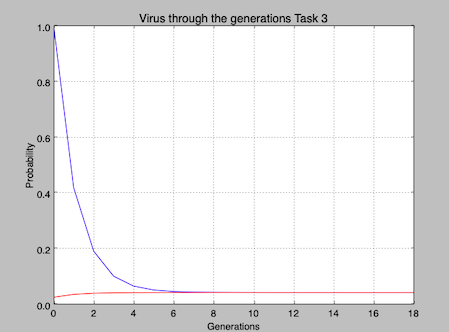
\includegraphics{plot_Markov}\\
		\item
		After 6 timesteps does the ratios stop to change significantly. Stable probability:
		\begin{equation}
								P_{} = 
\begin{pmatrix}
0,42 & 0,974\\
0,58 & 0,026

\end{pmatrix}
		\end{equation}
				\begin{equation}
								\overline{X} = 
\begin{pmatrix}
A\\
B

\end{pmatrix}
		\end{equation}
						\begin{equation}
								P* \overline{X} = \overline{X} \leftrightarrow \begin{pmatrix}
0,42 & 0,974\\
0,58 & 0,026

\end{pmatrix} * \begin{pmatrix}
A\\
B

\end{pmatrix} = \begin{pmatrix}
A\\
B

\end{pmatrix}
		\end{equation}
		\begin{equation}
		0,42 A + 0,5B = A \Rightarrow 0,5B = A - 0,42A 
		\Rightarrow B = \frac{ 25 }{ 29 } = 0,86
		\end{equation}
		
				\begin{equation}
				0,58A + 0,026B = B
		\end{equation}
		
				\begin{equation}
				A + B = 1 \Rightarrow A + 0,86 = 1 \Rightarrow A = 0,14
		\end{equation}
		
		We can see the probability converge to our solution.

		
		\end{enumerate}
		
	\end{answer}
		
	\end{question}

	
\end{questions}


	\exercise{Information Theory}
\begin{questions}
	
	%----------------------------------------------
	\begin{question}{Entropy}{5}		
	\begin{answer} 
			\begin{enumerate}
		\item \begin{equation}
 - 0,04 * {\log_2 0,04}  - 0,22 * {\log_2 0,22} - 0,67 * {\log_2 0,67} - 0,07 * {\log_2 0,07} = 1,3219   
\end{equation}
An average of 1 bit can be transmitted.
		\item 
		\begin{equation}
		H = ln(4) = 1,386 \approx 2
		\end{equation}
		Maximum of 2 bits per symbol can be transmitted using a set of four symbols. 
		The distribution over the symbols requires that at least the maximum is as great as that of all other members.
		\end{enumerate}
		
	\end{answer}
		
	\end{question}
	
\end{questions}


	\exercise{Bayesian Decision Theory}
\begin{questions}
	
	%----------------------------------------------
	\begin{question}{Optimal Boundary }{4}		
	\begin{answer} 
			\begin{enumerate}
		\item 
		Bayesian decision theory is a fundamental statistical approach to the problem of pattern classification based probabilities.
		\item The goal is to decide which class an example $x$ most likely belongs to.
		This is done by comparing the class posterior probabilities $p(C_i\mid x)$, which can be calculated by Bayes' theorem:
		\[
		p(C_i \mid x)=\frac{p(x\mid C_i)p(C_i)}{p(x)} \propto p(x\mid C_i)p(C_i)
		\]
		\item The decision boundary of two classes $C_1$ and $C_2$ is given by $p(C_1\mid x)=p(C_2\mid x)$, where  $C_1$ is chosen over $C_2$ if $p(C_1\mid x)>p(C_2\mid x)$.
		\end{enumerate}
		
	\end{answer}
		
	\end{question}
	
		%----------------------------------------------
	\begin{question}{Decision Boundaries  }{8}		
	\begin{answer} 
		Given that the propabilites and variances of the two classes are equal, the decision boundary should only be influenced by the two means, sitting centered between them.(x represents the boundary)
		\begin{equation}
		 (x-\mu_1)^2 = (x-\mu_2)^2 \\
		x = \frac{ (x-\mu_1)^2 = (x-\mu_2) }{Q * (\mu_1-\mu_2)}\\
		\end{equation}
		\begin{equation}
		If  \mu_1 = \mu_2 , No decision Boundary 
		\end{equation}

		\begin{equation}
		else: x =\frac{\mu_1 + \mu_2}{2}
		\end{equation}
			
	\end{answer}
		
	\end{question}
	
	%----------------------------------------------
	\begin{question}{Different Misclassification Cost }{8}		
	\begin{answer} 
		Given that wrongly identifying a case of $C_2$ as $C_1$ is more costly than the other way around, the Decision Boundary has to be moved towards $C_1$, causing samples to be more often identified as $C_2$ \\
		$ \mu_1>0; \mu_1=2*\mu_2; \delta_1=\delta_2; p(C_1)=p(C_2) \\\\
		4(2\pi *\delta_1^2)^{ \frac{-1}{2} } * \exp( -\frac{(x-\mu_1)^2}{2\delta_1^2} ) * p(C_1) 
		=(2\pi *\delta_2^2)^{ \frac{-1}{2} } * \exp( -\frac{(x-\mu_2)^2}{2\delta_2^2} ) * p(C_2)
		\\
		\\
		\log(4) + \frac{(x-\mu_2)^2}{2\delta_2^2} = \frac{(x-\mu_2)^2}{2\delta_2^2}
		\\
		\\
		2\mu_2^2 * x -3\mu_2^2 = -\log(4) * \delta_2^2
		\\
		\\
		x = \frac{3\mu_2^2 - \log(4) * 2\delta_2}{2\mu_2^2}
		$
	\end{answer}
		
	\end{question}
	
\end{questions}


	
\end{document}

